\section{Prohledávání do šířky}\label{sec:bfs}

Jednou ze základních úloh je procházení grafu z určitého vrcholu a zjištění dosažitelnosti ostatních vrcholů. Nejednodušším algoritmem v tomto ohledu je tzv. \emph{prohledávání do šířky} (angl. \emph{breadth-first search}, zkráceně BFS). Jeho základní princip spočívá v postupném objevování následníků již nalezených vrcholů. Na počátku dostaneme graf $G=(V,E)$ a nějaký počáteční vrchol $v_0\in V$. Postupně objevíme všechny sousedy vrcholu $v_0$, poté všechny sousedy těchto nalezených sousedů, atd. Na BFS lze nahlížet tak, že do počátečního vrcholu nalijeme vodu a sledujeme, jak postupuje vzniklá vlna.

Pro každý vrchol si budeme uchovávat jeho \emph{stav}.
\begin{itemize}
    \item \emph{Nenalezený} -- vrchol jsme ještě během výpočtu neviděli.
    \item \emph{Otevřený} -- vrchol jsme viděli, ale ještě nejsme neprozkoumali všechny jeho sousedy.
    \item \emph{Uzavřený} -- vrchol jsme prozkoumali společně se všemi jeho sousedy a dál se jím již netřeba zabývat.
\end{itemize}
Na počátku začneme s jedním otevřeným vrcholem a to $v_0$ (zde začínáme). Po prozkoumání všech sousedních vrcholů se jejich stav změní na otevřený a počáteční vrchol $v_0$ se uzavře. Obdobně pokračujeme pro nově otevřené vrcholy. Pokud by náhodou mezi dvojicí otevřených vrcholů existovala hrana, pak si sousedního vrcholu všímat nebudeme, neboť byl již otevřen. Pro každý vrchol se ještě dodatečně můžeme uchovávat informaci, jak daleko se nachází od $v_0$, co do počtu hran ležících na cestě.

\begin{pseudo}{BFS}{Graf $G=(V,E)$ a počáteční vrchol $v_0\in V$.}{Seznam vzdáleností $D$.}
    \Comment{Inicializace}
    \begin{For}{každý vrchol $v\in V$}
        $stav(v)\leftarrow$ \textit{nenalezený}\\
        $D(v)\leftarrow\infty$
    \end{For}
    $stav(v_0)\leftarrow$ \textit{otevřený}\\
    $D(v_0)\leftarrow 0$\\\\
    Založ frontu $Q$ a přidej do ní vrchol $v_0$\\
    \begin{While}{je fronta $Q$ neprázdná}
        $v\leftarrow$ první vrchol ve frontě $Q$, který z ní odebereme\\\\
        \Comment{Prozkomáváme všechny dosud neobjevené sousedy}
        \begin{For}{každý sousední vrchol $w$ vrcholu $v$}
            \begin{If}{$stav(w)=$ \textit{nenalezený}}
                $stav(w)\leftarrow$ \textit{otevřený}\\
                $D(w)\leftarrow D(v)+1$\\
                Přidej $w$ do fronty $Q$
            \end{If}
        \end{For}
        $stav(v)\leftarrow$ \textit{uzavřený}
    \end{While}
\end{pseudo}

BFS rozděluje vrcholy do vrstev podle toho, v jaké vzdálenosti od počátečního vrcholu se nachází (viz obrázek \ref{fig:bfs_vrstvy}). Nejdříve jsou prozkoumány vrcholy ve vzdálenosti 0 (tj. pouze $v_0$), poté ve vzdálenostech 1, 2, \dots Z toho vyplývá, že kdykoliv při otevírání libovolného vrcholu $v$ nastavujeme hodnotu $D(v)$, bude tato hodnota vždy odpovídat délce nejkratší cesty z $v_0$ do $v$. Tato hodnota bude však nastavena pouze u těch vrcholů, které jsou z $v_0$ dosažitelné (ostatní vrcholy zůstanou ve stavu nenalezený).
\begin{figure}[h]
    \centering
    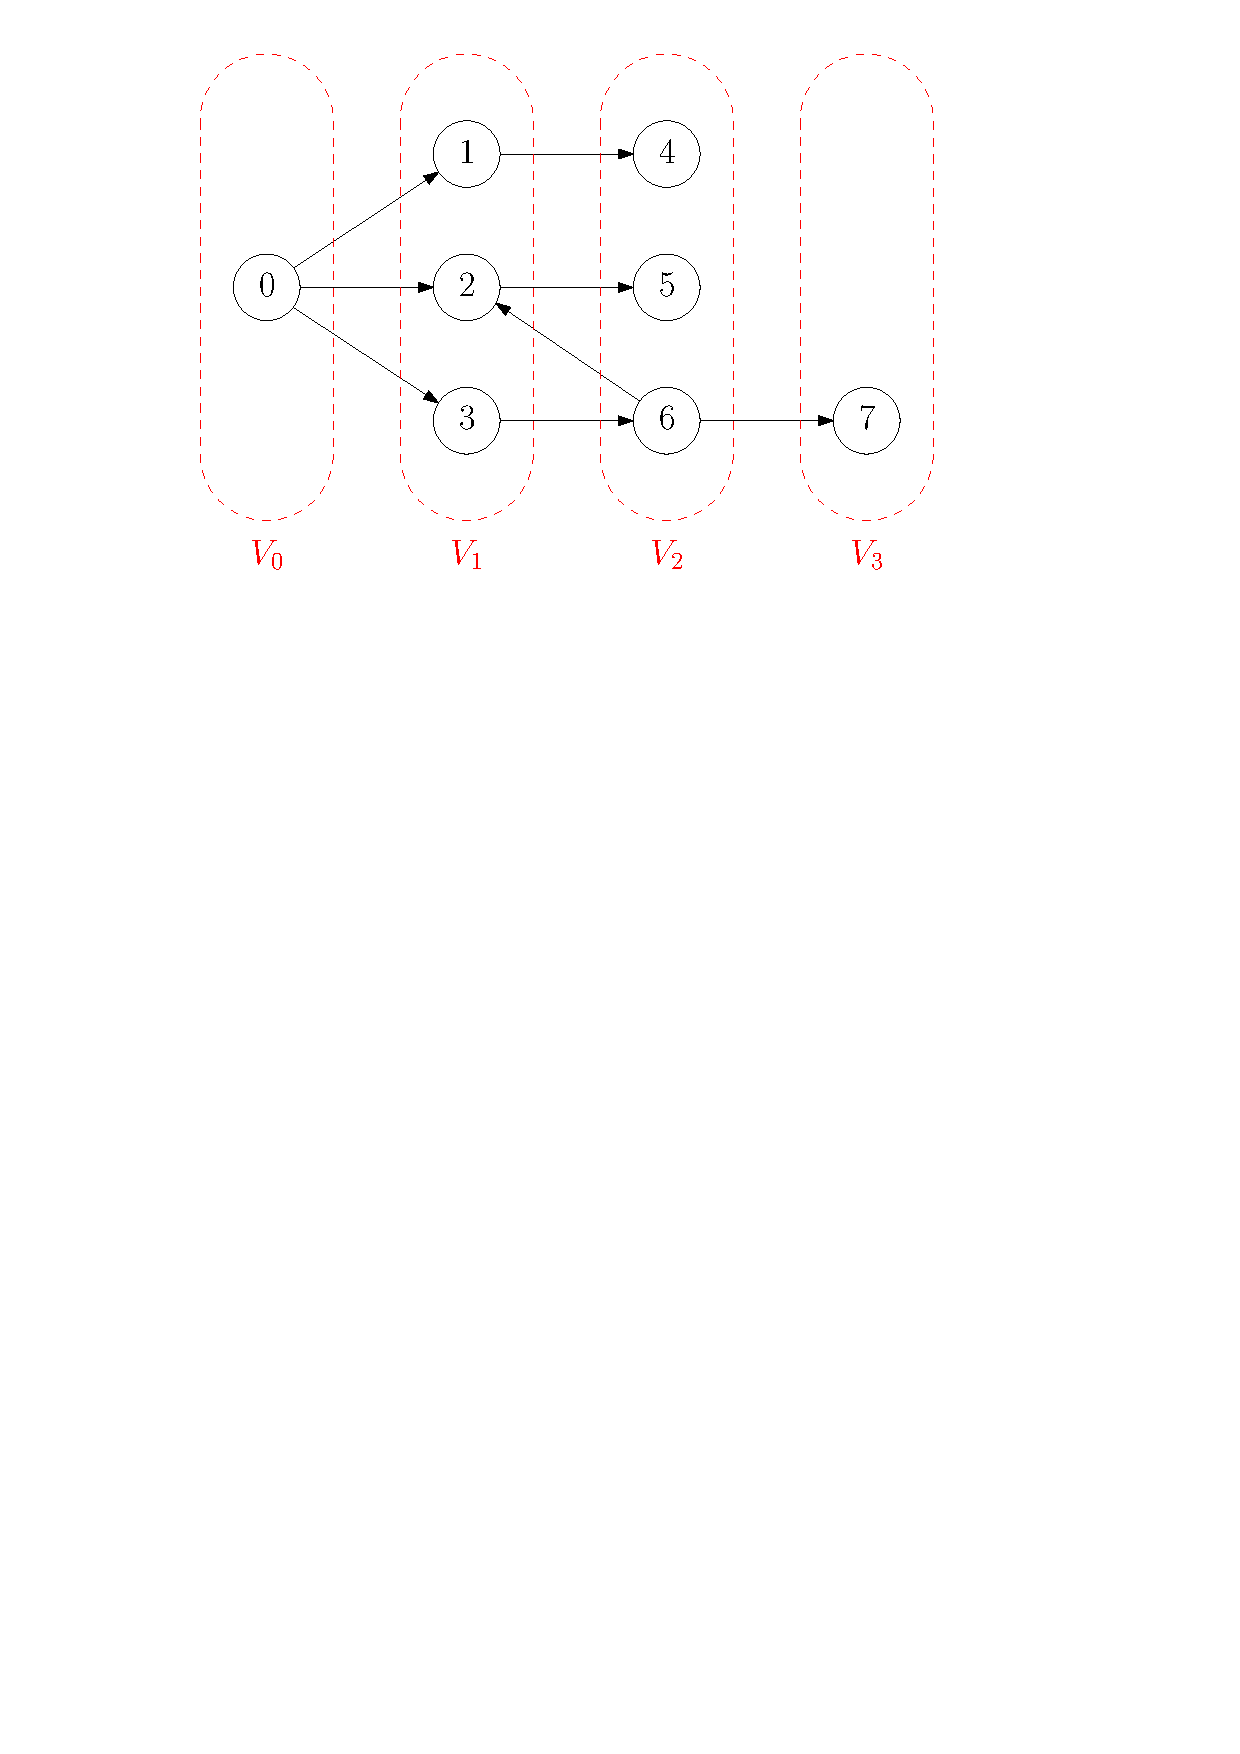
\includegraphics[scale=1]{ch01_bfs_vrstvy.pdf}
    \caption{Vrcholy rozdělené do vrstev podle průběhu BFS.}
    \label{fig:bfs_vrstvy}
\end{figure}

Zbývá prozkoumat časovou a paměťovou složitost BFS. Označme si počet vrcholů grafu $G$ na vstupu $n$ a počet jeho hran $m$. 
\begin{theorem}[Složitost BFS]\label{thm:bfs_slozitost}
    Algoritmus BFS doběhne v čase $\bigO{n+m}$ a spotřebuje paměť $\bigO{n+m}$.
\end{theorem}
\begin{proof}
    Inicializace potrvá $\bigO{n}$, neboť cyklus iteruje přes všechny vrcholy. Vnější cyklus provede maximálně $n$ iterací, protože každý z vrcholů uzavřeme nejvýše jednou, tj. $\bigO{n}$.

    S vnitřním cyklem je to trochu složitější, protože jeho počet iterací závisí na tom, který z vrcholů otevíráme (resp. na počtu jeho sousedů). To znamená, že pokud si označíme $d_i$ počet sousedů vrcholu $i$, pak celkový počet iterací vnitřního cyklu přes všechny vrcholy bude $\sum_i{d_i}$. Lze si ovšem všimnout jedné užitečné věci. Pokaždé, když prozkoumáváme sousední vrchol $w$ nějakého vrcholu $v$, mohou nastat dva případy podle toho, jestli je $G$ orientovaný graf, nebo neorientovaný.
    \begin{enumerate}[label=(\roman*)]
        \item\label{bfs_slozitost_neor_graf} Graf $G$ je neorientovaný. Pak hranu, která spojuje $v$ a $w$ prozkoumáme právě \emph{dvakrát} (jednou z vrcholu $v$ a podruhé z vrcholu $w$). Každá hrana se tak započítá dvakrát, tzn. vnitřní cyklus se celkově provede max $2m$-krát (po všech iteracích vnějšího cyklu).
        \item\label{bfs_slozitost_or_graf} Graf $G$ je orientovaný. Pak se hrana započítá pouze jednou, a to z vrcholu, z něhož vede. Celkově se vnitřní cyklus provede $m$-krát.
    \end{enumerate}
    V prvním případě tak pro časovou složitost bude platit
    \[\bigO{n+\sum_i{d_i}}=\bigO{n+2m}=\bigO{n+m}.\]
    V druhém případě dojdeme ke stejnému výsledku, akorát zmíněná suma bude, kvůli orientaci hran, rovna přesně počtu hran, tj.
    \[\bigO{n+\sum_i{d_i}}=\bigO{n+m}.\]
\end{proof}
\begin{figure}[h]
    \centering
    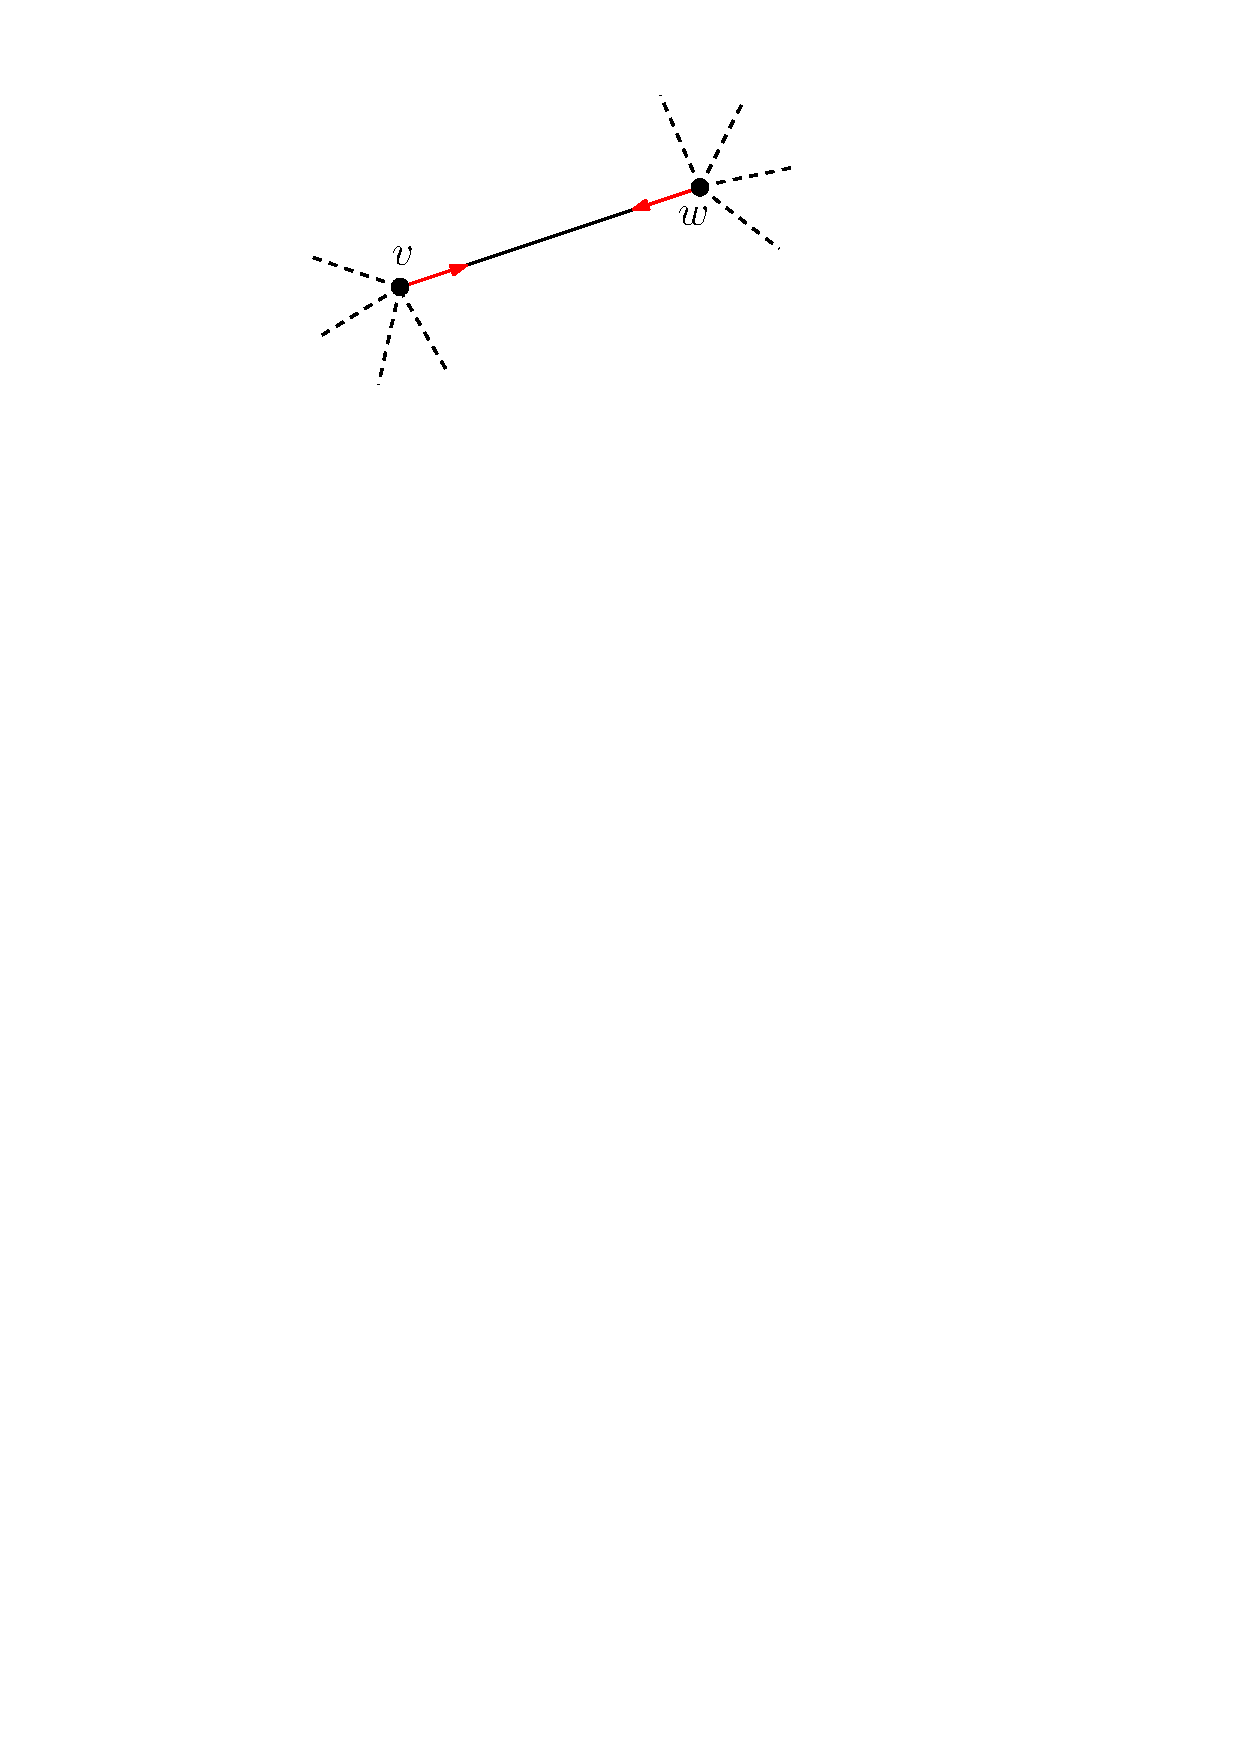
\includegraphics{ch01_zapocitavani_hran.pdf}
    \caption{Znázornění situace v důkazu části \ref{bfs_slozitost_neor_graf} věty \ref{thm:bfs_slozitost}.}
\end{figure}